\documentclass[a4paper, 10pt]{article}

%==============================================================================%
%--------------------------------     Intro     -------------------------------%
%==============================================================================%

% Tout document LateX commence par la commande "documentclass".  Elle spécifie
% à LaTeX le type de document que tu essaie de produire.  Dans notre cas (et
% dans 90% des cas), on produis un article.  Nous avons ausi spécifié que nous
% voulons un grosseur d'écriture de 11 points.


%==============================================================================%
%-------------------------     Structure Générale     -------------------------#
%==============================================================================%

% Un document LaTeX est composé de deux grandes parties:
%   - Le préambule
%   - Le document

% Préambule: Cette section contient tout ce qui n'apparait pas directement
% dans le document. C'est ici par exemple que tu spécifie des informations
% comme le titre et l'auteur. Tu veux mettre en place un racourcis qui t'évite
% de réécrire des longs mots? Tu le mets ici. Tu veux changer l'apparence
% globale des sections de ton document, tu le configure ici. Tu veux utiliser
% divers sous-programmes (appelé librairies) pour ajouter à ton document
% (comme par exemple insérer des images)? C'est aussi ici. C'est utile
% d'organiser cette section en placant les informations cruciales sur ton
% document (titre, auteur, etc...) au tout début, suivit des sous-programmes
% que tu installes puis mettre tout le reste ensuite.

% Document:
% C'est ici que tu formatte écris ton texte.


%==============================================================================%
%-------------------------------     La Base     ------------------------------%
%==============================================================================%

% LateX fonctionne avec des commandes, celles-ci sont délimitées par le "\".
% Il existe différents types de commandes:
%   - Les commandes en-ligne SANS arguments
%   - Les commandes en-ligne AVEC arguments
%   - Les commandes en blocs
%    - Les commentaires
% Si tu désire absolument écrire le charactère "\" dans ton document, tu dois
% utiliser la commande "\textbackslash"

% Commandes en-ligne SANS arguments:

% Ce sont des commandes qui n'ont besoin d'aucune information pour
% fonctionner. Quelques exemples sont: today (écris la date d'aujourd'hui),
% maketitle (Génère la page de présentation), newpage (crée une nouvelle page)
% et tableofcontents (génère la table des matières). Leur structure va comme
% suit:
%   \commande
% Donc avec la même logique, les commandes précédentes seraient:
%   \today
%   \maketitle
%   \newpage
%   \tableofcontents

% Commandes en-ligne AVEC arguments:
% Certaines commandes ont besoin d'informations pour fonctionner. Notament,
% comment LaTeX mettrait-il quelquechose en gras si tu ne lui dis pas où
% commencer et oû arrêter? D'autres commandes peuvent avoir des options en
% plus. LaTeX prends des données pour acquis. Mais si tu veux qu'il agisse
% différement, tu lui spécifie. La structure va comme suit:
%   \commande[option]{argument}
% Voici quelques exemples de commandes sans options:
%    \textbf{Texte en gras}
%    \textit{Texte en italiques}
%    \cite{code_pour_une_citation}
%    \ref{code_pour_une_figure}
% Voici un exemple d'une commande avec options; Celle-ci inclue une image dans
% ton document:
%     \includegraphics[width=5cm, angle=45]{chemin/vers/image.png}
% Il serait tout à fait correct d'écrire la dernière commande sans options:
%     \includegraphics{chemin/vers/image.png}
% Alors, l'image serait intégré dans sa résolution initiale. Les options
% permettent de spécifier certains paramètres d'une commande. Ici, la commande
% avec options spécifie une orientation de 45 degrés (angle=45) et  une
% largeur de 3cm (width=3cm).

% Les Commentaires:
% Comme tu le vois, j'écris beaucoup de texte ici qui ne semble pas être lu
% par LaTeX. Tout ce qui suit le symbole "%" dans un doument est ignoré par
% LaTeX.  Pour écrire le sybole "%" dans ton document, tu dois le précéder
% d'un "\" comme si c'était une commande.


%==============================================================================%
%----------------------------     Informations     ----------------------------%
%==============================================================================%

\title{Une Introduction à \LaTeX}
\author{Benjamin Chausse}
\date{\today}


%==============================================================================%
%------------------------------     Packages     ------------------------------%
%==============================================================================%

\usepackage{graphicx}            % Pour insérer des images
\usepackage{float}               % Pour facilement positionner des images
\usepackage[T1]{fontenc}         % Pour des charactères français compatibles
\usepackage[french]{babel}       % Pour un formatage en français
\usepackage[hidelinks]{hyperref} % Pour pouvoir clicker des éléments
\usepackage{xcolor}              % Pour utiliser des couleurs
\usepackage{amsmath}             % Pour des équations mathématiques


%==============================================================================%
%-------------------------------     Autres     -------------------------------%
%==============================================================================%

% Préférence pour afficher du code (Ne t'en fais pas pour le tutoriel)
\definecolor{codebackground}{HTML}{DFDFED}

%==============================================================================%
%-------------------------     Début du document     --------------------------%
%==============================================================================%

\begin{document}

% Créons une page de présentation:
\maketitle

% Ajoutons un résumé à la première page:
\abstract{
Comment utiliser \LaTeX? Ce document expliquera les bases nécessaire à une
utilisation rudimentaire de ce programme aux possibilités sans fin.
Son code source est très commenté. Il est préférable de le consulter en tandem
avec ce pdf pour maximiser sa compréhension.
}

% On veut commencer la table des matières sur une nouvelle page:
\newpage

% Créons une table des matières:
\tableofcontents

% On veut avoir le reste du document sur une nouvelle page:
\newpage

% Créons la première section de notre document:
\section{Formattage de base} Avant de se lancer dans les fonctions plus
complexes de \LaTeX, il faut comprendre la base. Je vai commencer par expliquer
la commande \verb+\verb+ pour éviter toute confusion. C'est une fonction
servant à exprimer une commande \LaTeX dans le pdf final sans qu'elle ne
s'exécute lorsque je l'écris afin de me faciliter la tâche dans l'écriture de
ce document. Elle formate aussi le look de certaines des commandes qui
apparaissent textuellement dans le pdf afin qu'elles aient une typographie
différente (comme du code), et par conséquent, plus apparentes.

Bon, maintenant à l'essentiel. Comme tu l'as vu, pour commencer un nouvelle
secion, tu utilise la commande \verb+\section+. Elle sont numérotés
automatiquement et sont automatiquement placées dans la table des matières.
Il est possible d'ajoutter deux dimensions supplémentaire aux document avec
les commandes \verb+\subsection+ et \verb+\subsubsection+ comme suit:

\subsection{Ceci est une sous-section}
\subsubsection{Ceci est une sous-sous-section}

Toutefois, il existe aussi des commandes pour formatter du texte à l'intérieur
d'un paragraphe.

\subsection{Formatage dans un paragraphe}

J'aimerais mentionner la commande \verb+\textbackslash+. Celle-ci de
permet d'exécuter un retour à la ligne. Ceux-ci sont utile pour accentuer la
distance entre deux paragraphe. \\

Pour écrire du texte en gras, il est possible d'utiliser la commande
\verb+\textbf+. En voici \textbf{un exemple}. Il est aussi possible
d'écrire du texte en italique avec \verb+\textit+ comme tu le
\textit{vois ici}. Il peut aussi être intéressant d'avoir des listes numérotés
dans un document. Cela peut être fait avec les balises
\verb+\begin{enumerate}+ et \verb+\end{enumerate}+:

\begin{enumerate}
  \item Premier éléments
  \item Chaque élément commence par \verb+\item+
  \item Troisième élément
  \item Cela permet d'avoir des
    éléments qui s'étalent
    sur plusieures lignes comme ici.
  \item Ciquième élément \\
\end{enumerate}

Les listes non-numérotées sont assez similaires. On n'a qu'à remplacer
"enumerate" par "itemize" puis le tour est joué:

\begin{itemize}
  \item Premier éléments
  \item Deuxième élément
  \item Troisième élément \\
\end{itemize}

Une dernière commande assez importante à mon avis est celle qui permet de
centrer certains éléments. Tu le fais avec les balises \verb+\begin{center}+
et \verb+\end{center}+

\begin{center}
Prends cette phrase comme exemple.
\end{center}

Cela sera surtout utile pour des équations, des tableaux, et des figures
mais je te la montre maintenant puique cela me semble le plus opportun.

\subsection{Les équations}

Les équations sont une partie extrêmement utile de \LaTeX.
Elle sont facilement modifiable et ne demandent pas de chercher des symbole
dans des menus comme dans word. Si tu désires écrire une équations
au beau milieu d'un paragraphe, comme par exemple $E=mc^2$, tu peux le faire
à en entourant ton équation de deux "\$" (vois les comme des parenthèses).

\subsubsection{Les équations simples}
Parfois tu peux vouloir donner à une équation un peux plus d'inportance.
Alors, tu peux la mettre dans la banière \verb+\begin{equation}+,
\verb+\end{equation}+. Elle sera alors sortie du paragraphe et indexée
à l'aide d'un numéro entre parenthèses (à droite). Par exemple:

\begin{equation}
  F = \dfrac{ G m_1 m_2 }{ R^2 }
\end{equation}

L'avantage que tu retires de procédér comme cela est que tu pourra
plus tard faire référence à ton ton équation et même lui donner un
titre (Nous en parlerons dans les "floats"). Par exemple:

\subsubsection{Les équations en chaines}
Parfois, tu veux développer ton raisonnement mathématiques sur plusieures
lignes. À ce moment, il existe une autre façon assez élégante avec \LaTeX
de présenter le tout. Voici un exemple:

\begin{align}
  f(x) &= \int{42x^2 } dx \\
  f(x) &= 42\int{x^2 } dx \\
  f(x) &= 42 \cdot \dfrac{x^3}{3} + C
\end{align}

Note comment tout les signes d'égalité sont alignés. En fait le symbole "\&"
devant le signe d'églité agit comme un séparateur pour une colonne dans un
tableau. Cela rend le tout beacoup plus esthétique quand tu as plusieurs
signes d'égalité sur la même ligne:

\begin{align}
  4a  &= 11b  & -6c  &= \dfrac{\pi}{2}d & 15e      &= 9f \\
  12a &= -17b & 24c  &= \dfrac{5}{\pi}d & 22e      &= -5f \\
  6a  &= -9b  & 14c  &= \pi d           & \sqrt{e} &= \dfrac{1}{f}
\end{align}

\subsubsection{Commandes utiles pour les équations}

\subsubsection{Symboles grecs (fais attention aux majuscules)}

\begin{itemize}
  \item \verb+\Delta+: $\Delta$
  \item \verb+\delta+: $\delta$
  \item \verb+\Gamma+: $\Gamma$
  \item \verb+\gamma+: $\gamma$
  \item \verb+\theta+: $\theta$
  \item \verb+\pi+   : $\pi$
\end{itemize}

\subsubsection{Outils mathématiques}

\begin{itemize}
  \item \verb+a^{exp}+:
      $a^{exp}$
  \item \verb+a_{indice}+:
      $a_{indice}$
  \item \verb+\dfrac{numerateur}{denominateur}+:
      $\dfrac{numerateur}{denominateur}$
  \item \verb+\sqrt{racine}+:
      $\sqrt{racine}$
  \item \verb+\int_{min}^{max}{interieur}+:
      $\int_{min}^{max}{interieur}$
  \item \verb+\left(interieur\right)+:
      $\left(interieur\right)$
  \item \verb+\textrm{texte normal}+:
      $\textrm{texte normal}$
\end{itemize}

\section{Les floats}

Les floats sont un concept vraiment utile dans \LaTeX. Elles permettent de
regrouper ensemble certains éléments pour qu'ils aient environ la même
esthétique et soient faciles à répérer.

\subsection{Les images (figures)}

Un des floats les plus facile à utiliser est la figure. Elle ne contient
qu'une image et son titre (qui est numéroté). Pour afficher un titre la
commande \verb+\caption{}+. Il est possible de faire référence à une
figure en utilisant la commande \verb+\label{}+ pour lui donner un
identifiant. Prends cet exemple:

\begin{figure}[H]
  \begin{center}
    \caption{Une image quelconque}
    \label{fig:xkcd}
    \includegraphics[width=5cm]{image.png}
  \end{center}
\end{figure}

Ici j'ai inséré une images (qui est dans le même dossier que mon fichier
\LaTeX). Elle provient d'une bande dessinée sur internet nommée \textit{XKCD}.
Je lui ai donc donné la référence ``fig:xkcd'' ce qui m'informe, moi (pas
l'ordinateur), de deux chose:

\begin{enumerate}
\item
  C'est une figure (d'où le préfixe fréquement utilisé ``fig'')
\item
  Ce qui la rend unique est qu'elle vient de \textit{XKCD}
  (bref, une information qui la rend unique, facile à citer).
\end{enumerate}
Pour utiliser la référence que je me suis donné, je peux utiliser la commande
\verb+\ref{}+. Ainsi, je peux écrire:

\begin{center}
Comme on le voit dans la figure \ref{fig:xkcd}, les priorités de notre société
ne sont pas toujours les meilleurs\ldots
\end{center}

Tu peux voir dans le fichier ``.tex'' original que le numéro un s'est écrit
automatiquement avec la commande \verb+\ref{fig:xkcd}+. Le numéro s'ajuste
automatiquement si le numéro de la figure change.

\subsection{Les tableaux}

\section{Les Citations}


\end{document}
